%!TEX root = main.tex

\chapter{Introducción}

La web actual está hecha por y para las personas. Desde las publicaciones en las
redes sociales hasta los artículos más avanzados en las enciclopedias virtuales
son formas de transferir información entre individuos y por ello utilizan el
lenguaje natural para hacer más fácil su entendimiento. Si bien estas
características facilitan la comprensión para el ser humano, hacen cada
vez más difícil el manejo de estos datos por parte de las computadoras.

La web semántica nace como forma de solucionar esta problemática. Su objetivo es
la creación de tecnologías que logren que tanto computadoras como personas
puedan interpretar y procesar la información almacenada en Internet
de forma simple.

Uno de los pilares fundamentales para la creación de una web en la cual toda
información pueda ser accedida por computadores de manera rápida y efectiva es
la generación de datos enlazados, es decir, la integración y publicación del 
conocimiento existente a un modelo que permita la interconexión y extensión de
los datos sin limitar el dominio ni las relaciones de los mismos.

Actualmente existe una gran cantidad de datos de libre acceso enlazados en la
web. La figura \ref{fig:cloud} muestra un esquema de ellos y provee una visión
global de los diferentes tópicos que estos datos tratan, ya sean datos
geográficos, de redes sociales, biológicos o lingüísticos (entre otros).

Pero, ¿Cuales son los datos más importantes para los usuarios?, ¿Cómo se
relacionan entre ellos? Son interrogantes que se presenta naturalmente al
momento de evidenciar la cantidad abrumadora de datos enlazados existentes.
En este trabajo se intentará responder dicha interrogante para los datos de
DrugBank, parte el proyecto Bio2RDF, el componente más importante de los datos
enlazados de índole biológica.

\begin{figure}[ht]
  \centering
  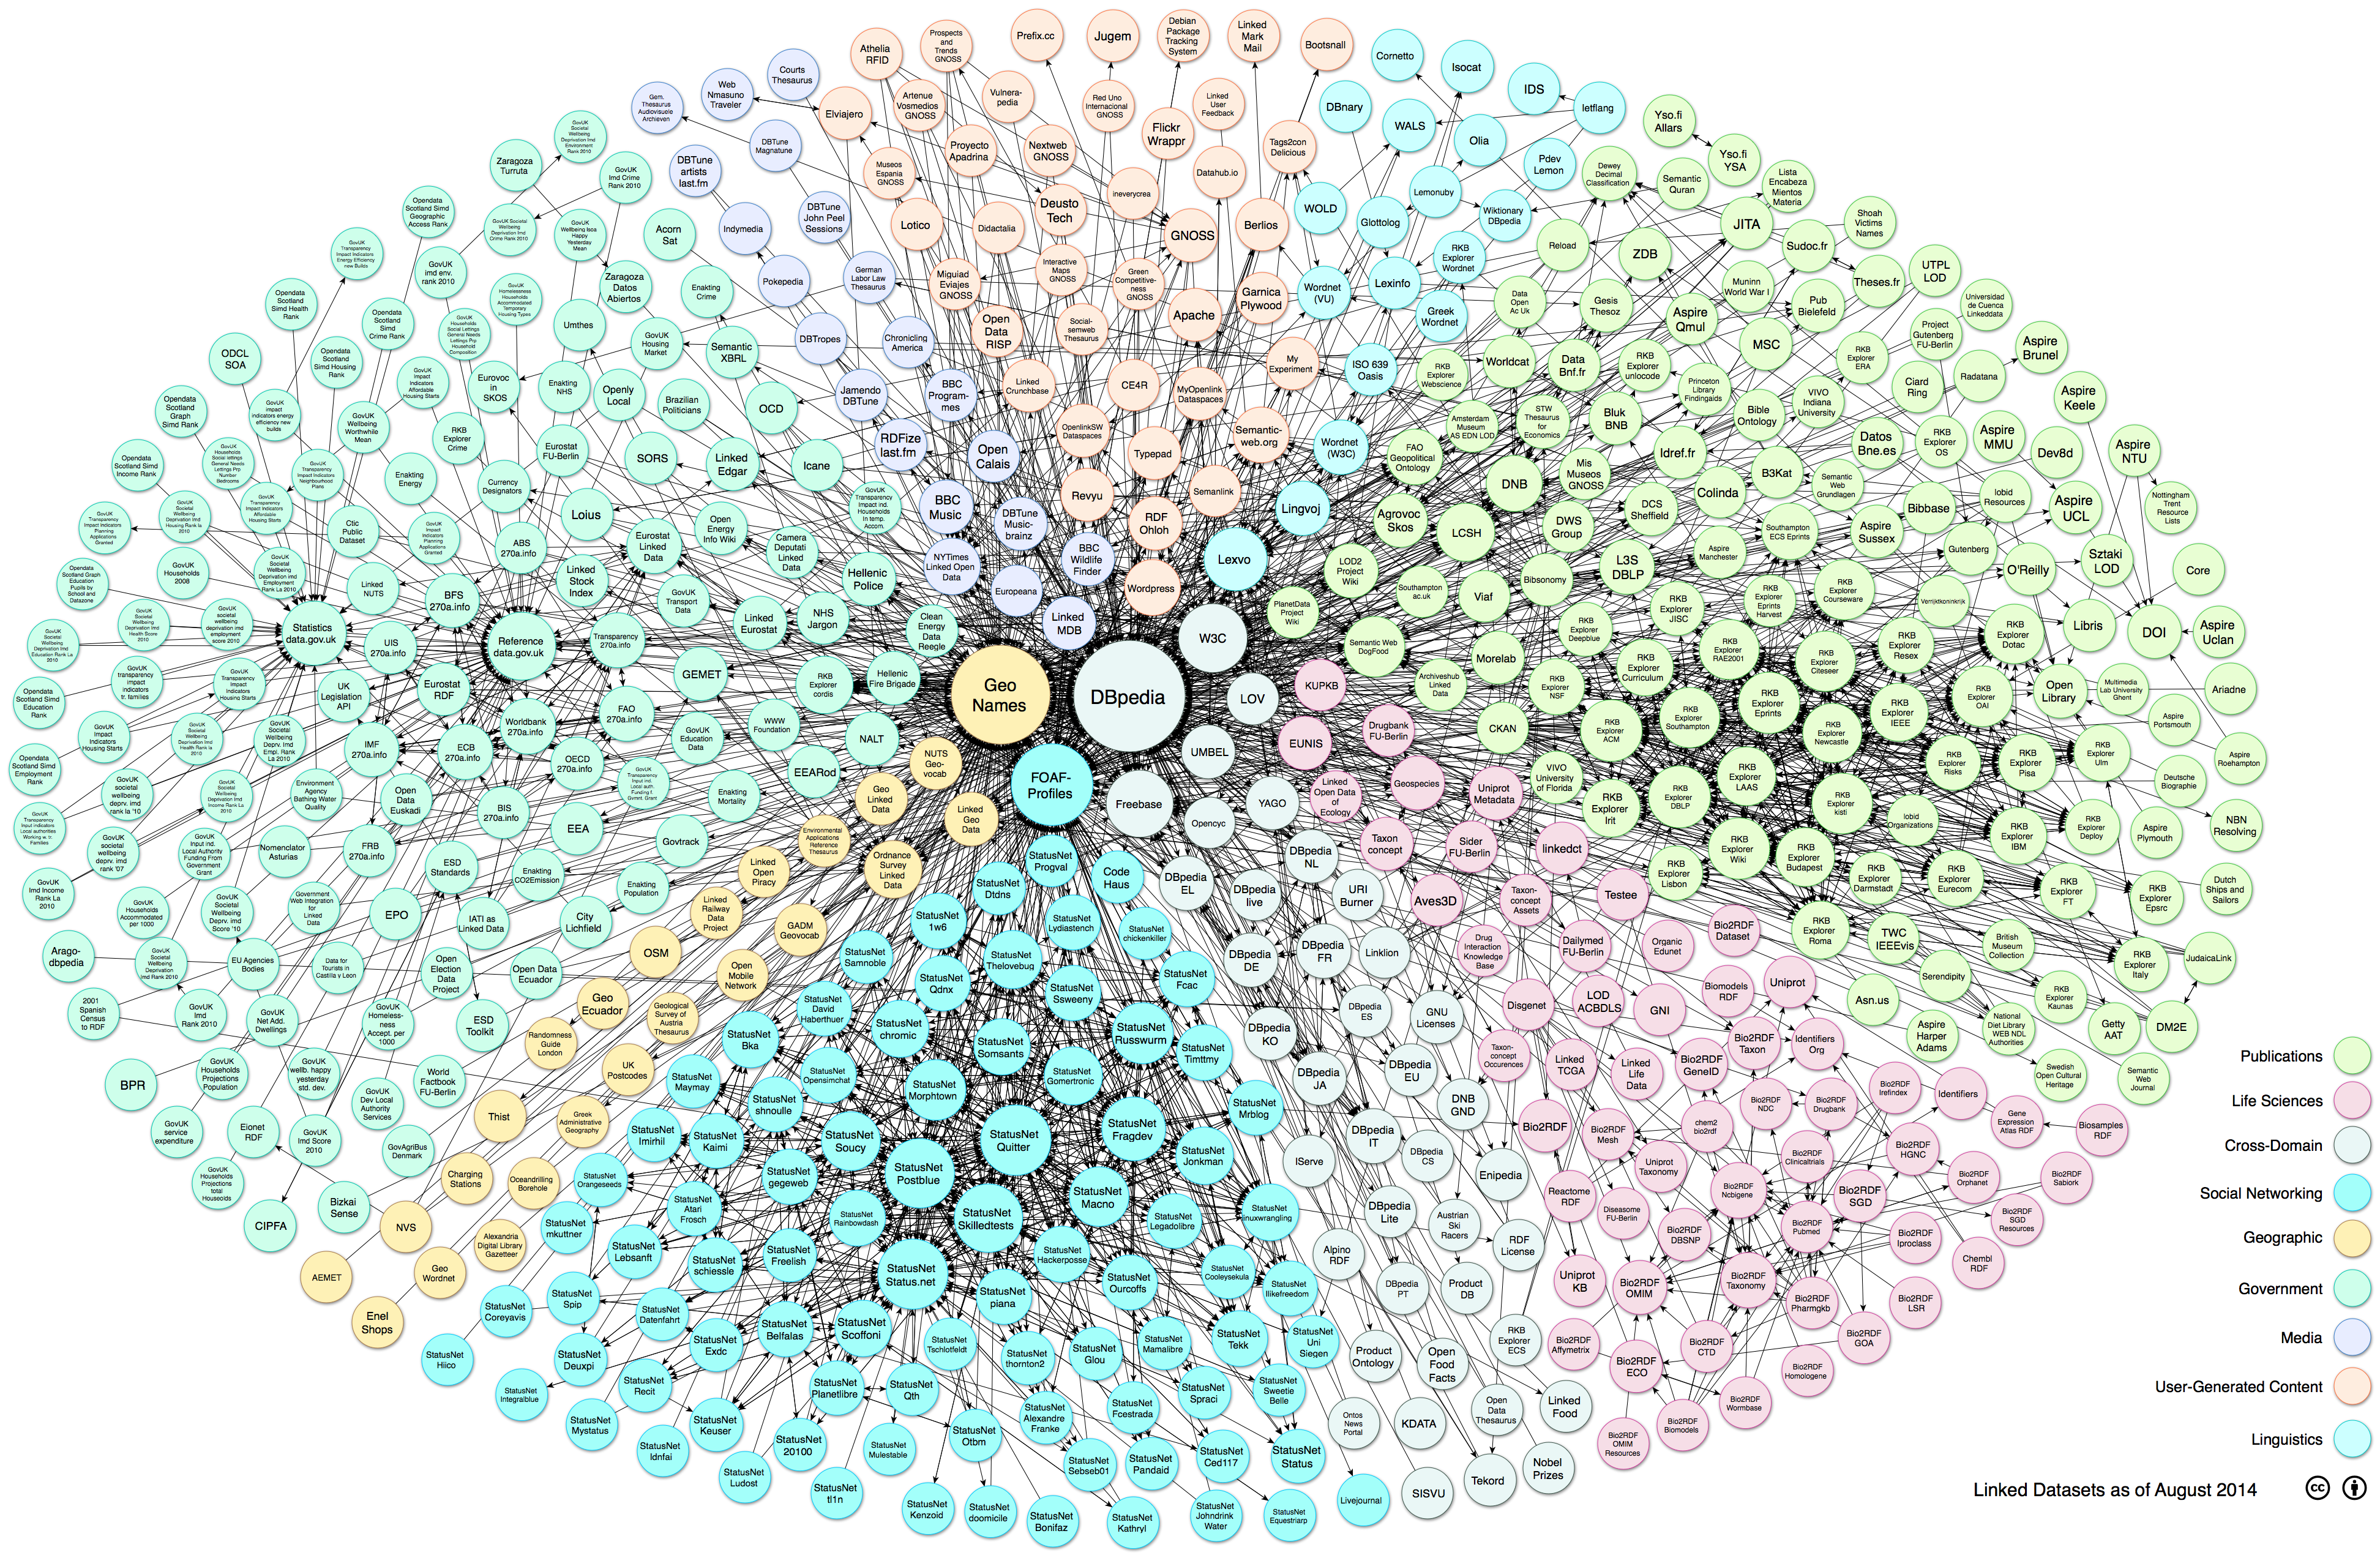
\includegraphics[width=\textwidth]{figures/open_linked_data_could.png}
  \caption{Conexiones entre las bases de datos abiertas hasta agosto del 2014.}
  \vspace{-.2cm}
  \caption*{En morado las bases de datos biológicas, gran parte de ellas son
  parte del proyecto Bio2RDF.}
  \vspace{-.2cm}
  \caption*{Creado por Linked Open Data Cloud project\cite{lod:cloud}.}
  \label{fig:cloud}
\end{figure}
~\vspace{-1cm}
\section{Identificación del problema}

El proyecto Bio2RDF (en su versión 3) incorpora la información de 35 bases de
datos RDF con información biológica, cerca de 11.000 millones de triples que
conforman la red de data enlazada más grande de esta ciencia.

Debido al volumen de datos que se manejan en este proyecto se hace interesante
determinar cual es la información más consultada por parte de los usuarios y 
así verificar que ésta tenga el soporte adecuado en el modelo. 
Para ello es indispensable contar con métricas que analicen el uso de los datos
consultados y la relación entre los mismos.

Si bien en trabajos anteriores como en Hu \emph{et al.}\cite{hu2015link} se han
determinado parámetros como el grado de distribución, la simetría y la
transitividad de los enlaces entre las diferentes bases de datos, no existe un
estudio que determine cual es el subconjunto de datos que realmente son
consultados por los usuarios y la relación entre estos y por ello no es posible
verificar cuales son las entidades más importantes dentro del proyecto Bio2RDF.

Se ha determinado (\hspace{1sp}\cite{hu2015link}) que los enlaces entre
las bases de datos de Bio2RDF presentan el fenómeno de ``mundo pequeño'' lo cual
indica que, a pesar del gran número de nodos que existen en esta red de datos,
generalmente es posible encontrar un camino relativamente corto entre ellos.
Este fenómeno se presenta generalmente en las redes sociales donde se
teoriza que dos individuos cualquiera están relacionados entre si por un número
pequeño de pasos, como describe la hipótesis de los seis grados de separación o
muestra el estudio ``Anatomy of Facebook''\cite{ugander2011anatomy}.

Debido a estas características consideramos atractivo generar un cálculo de
centralidad para los datos consultados por los usuarios al proyecto Bio2RDF,
específicamente a la base de datos que presenta mayor cantidad de consultas en
él: DrugBank, y de esta manera identificar cuales son las instancias más
importantes dentro de esta base de datos.

\section{Objetivos}

El objetivo de este trabajo es generar estadísticas de centralidad sobre el
subconjunto de datos consultados por los usuarios al proyecto Bio2RDF,
particularmente a la base de datos con más consultas en él: DrugBank y comparar
estos resultados con el modelo del proyecto en sí.

\subsection{Objetivos específicos}
Para el logro del objetivo general se plantean los siguientes objetivos
específicos:
\begin{enumerate}
  \item
    Generar un subgrafo del proyecto Bio2RDF a través del análisis de las
    consultas SPARQL hechas al servidor por parte de los usuarios en un periodo
    de tiempo determinado.
  \item
    Analizar el grafo generado por medio de métricas de centralidad para grafos.
  \item
    Comparar los resultados del estudio con el proyecto Bio2RDF.
\end{enumerate}
